%%%
%
% $Autor: Wings $
% $Datum: 2021-05-14 $
% $Pfad:  $
% $Dateiname: ListOfMaterial
% $Version: 4620 $
%
% !TeX spellcheck = de_DE/GB
% !TeX program = pdflatex
% !BIB program = biber/bibtex
% !TeX encoding = utf8
%
%%%




\chapter{Bill of Material}

%------------------------------------------------

% HARDWARE SECTION

%------------------------------------------------

\subsection{Hardware Bill of Materials}

The following hardware components are required to execute the CPI forecasting project. 
The hardware listed below provides a complete development environment for data analysis, 
model training, and result visualization.

\begin{table}[H]
	\centering
	\renewcommand{\arraystretch}{1.8} % Adds more vertical spacing between rows
	\begin{tabular}{|>{\centering\arraybackslash}m{4.2cm}|m{3.5cm}|m{1.7cm}|m{3.5cm}|m{2cm}|}
		\hline
		\textbf{Materials} & \textbf{Description} & \textbf{Quantity} & \textbf{Link} & \textbf{Price} \\
		\hline
		
		\makecell{\rule{0pt}{1.0cm}
\includegraphics[width=3.2cm]{../../Images/BOM_SBOM/laptop.png}} &
		A standard personal Laptop capable of running data analysis &   1    &
		\href{https://www.amazon.de/HP-Display-i5-1334U-Graphics-Windows/dp/B0DNTL5ZZP}{Laptop} &
		500 € to 1000 € \\
		\hline
		
		\makecell{\rule{0pt}{1.5cm}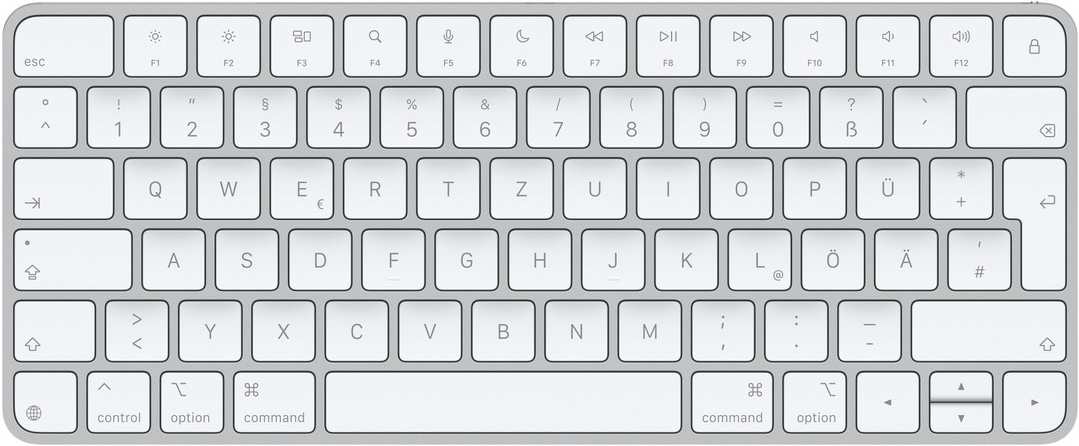
\includegraphics[width=3.0cm]{../../Images/BOM_SBOM/keyboard.jpeg}} &
		Keyboard. &   1    &
		\href{https://www.amazon.de/Logitech-G213-Gaming-Tastatur-Prodigy-RGB-Hintergrundbeleuchtung-Deutsches-Tastaturlayout/dp/B01L6L46LK}{Keyboard} &
		29.58 € \\
		\hline
		
		\makecell{\rule{0pt}{1.0cm}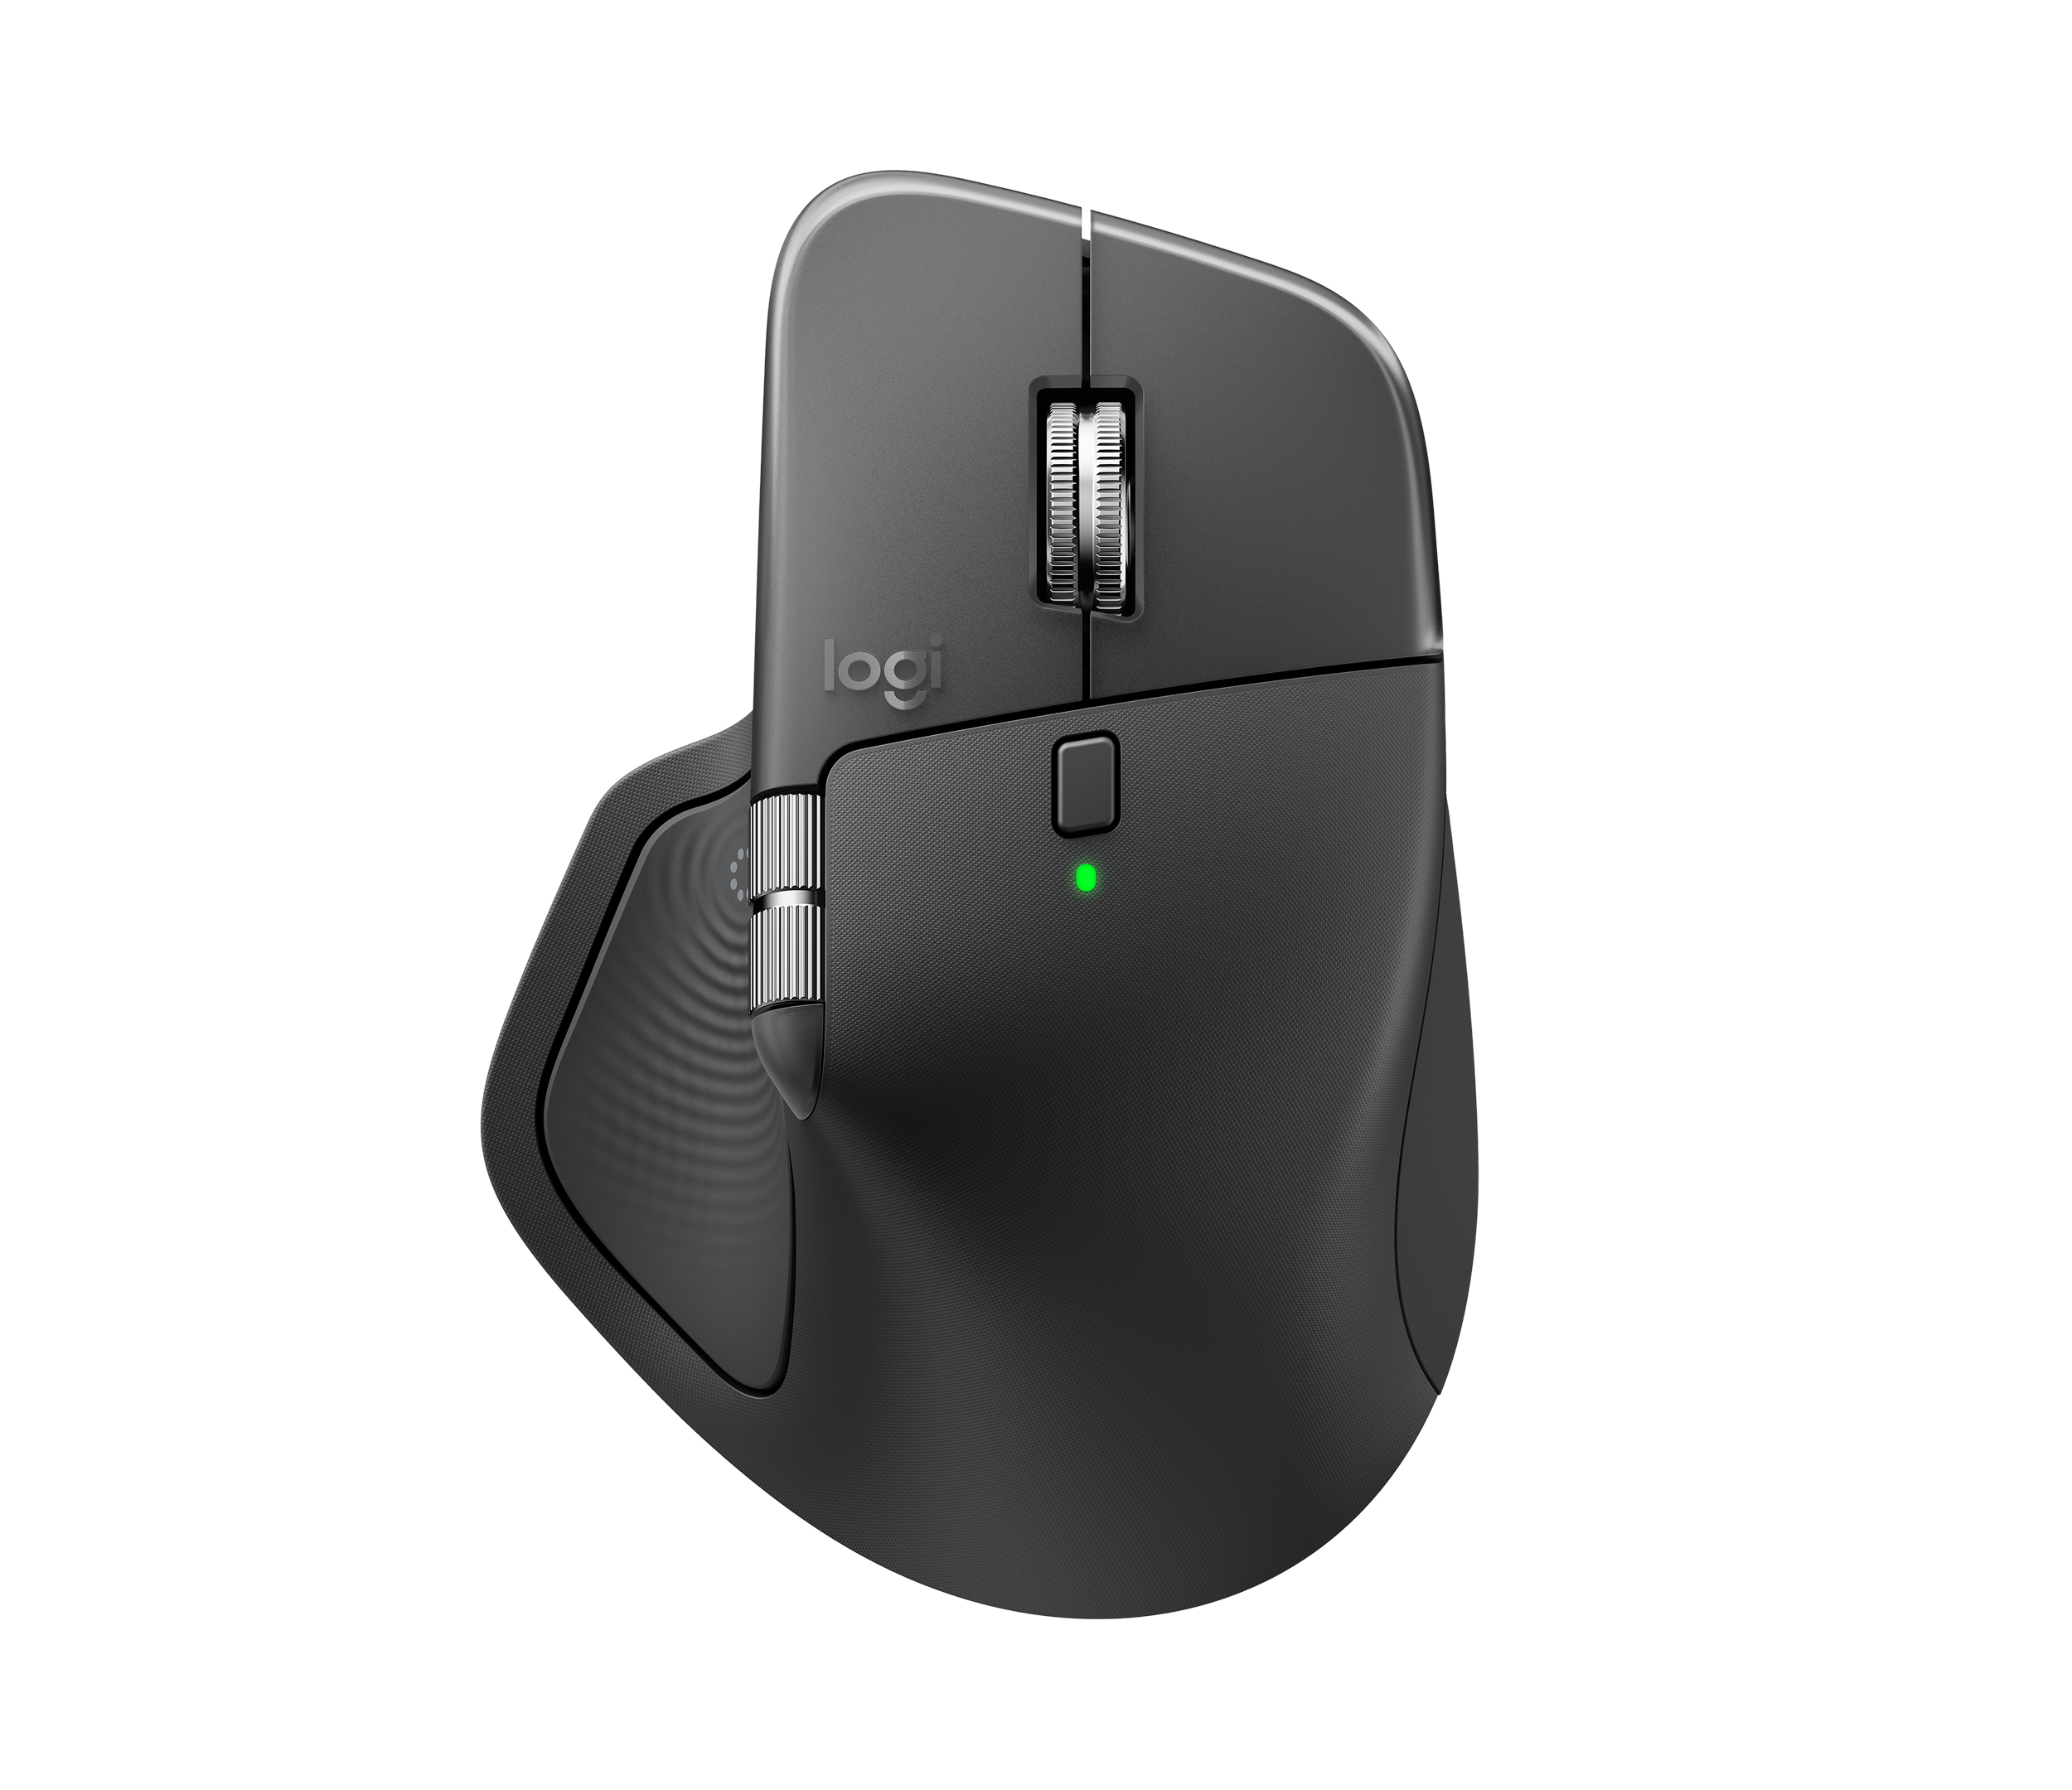
\includegraphics[width=3.0cm]{../../Images/BOM_SBOM/mouse.png}} &
		Mouse. &   1    &
		\href{https://www.amazon.de/Logitech-USB-Nano-Empf%C3%A4nger-Batterielaufzeit-Rechtsh%C3%A4nder-Kompatibel/dp/B00552K0GM}{Mouse} &
		7.49 € \\
		\hline
		
	\end{tabular}
	\caption{Hardware Bill of Materials}
	\label{Table 5.1}
\end{table}

\subsection{Laptop}

The laptop is the primary hardware component used to execute the CPI forecasting project. 
It provides the computational resources necessary for running the Python environment, 
performing statistical modelling, and generating visualizations.

\begin{itemize}
	\item Brand and Model: Dell XPS / Lenovo ThinkPad / MacBook Pro
	\item Processor: Intel Core i5/i7 or AMD Ryzen 5/7
	\item RAM: Minimum 8GB (16GB recommended)
	\item Storage: 512GB SSD minimum
	\item Operating System: Windows 10/11, macOS, or Linux
	\item Display: 15'' Full HD (1920x1080) or higher
\end{itemize}

\subsection{Keyboard}

An external keyboard improves typing efficiency and ergonomics during coding and report writing.

\begin{itemize}
	\item Brand and Model: Keychron K2
	\item Type: Wireless mechanical keyboard
	\item Connectivity: Bluetooth / USB-C
	\item Layout: Tenkeyless
	\item Battery: Rechargeable battery
\end{itemize}

\subsection{Mouse}

A mouse enhances navigation efficiency when working with development tools and visualizations.

\begin{itemize}
	\item Brand and Model: Logitech MX Master Series
	\item Type: Wireless optical mouse
	\item Connectivity: Bluetooth / USB receiver
	\item Battery: Rechargeable battery
	\item Ergonomics: Designed for long working sessions
\end{itemize}

\subsection{Hardware Note}

The CPI forecasting project is a software-first application. The computational requirements are modest: the dataset contains only 422 monthly observations, and the models (ARIMA, ETS, SARIMA) are classical statistical methods that do not require GPU acceleration or large amounts of memory. Any standard laptop or desktop computer from the last five years is sufficient for development, training, and deployment. The hardware BOM is therefore included for completeness, but it is not a critical project constraint.
